\documentclass[letterpaper,11pt] {article}
\usepackage{float} %forcing figures
\usepackage{amsmath,amsthm,amssymb}
\usepackage{tabularx} % extra features for tabular environment
\usepackage{amsmath}  % improve math presentation
\usepackage[makeroom]{cancel} %cancelling terms
\usepackage{graphicx} % takes care of graphics including machinery
\usepackage[margin=1in,letterpaper]{geometry} % decreases margins
\usepackage{witharrows}
\usepackage{caption} 
\captionsetup[table]{skip=10pt}
\usepackage[final]{hyperref} % adds hyperlinks inside the generated pdf file
\hypersetup{
	colorlinks=true,       % false: boxed links; true: colored links
	linkcolor=blue,        % color of internal links
	citecolor=blue,        % color of links to bibliography
	filecolor=magenta,     % color of file links
	urlcolor=blue         
}
\usepackage[colorinlistoftodos]{todonotes} %Add inline or margin comments to your PDF
\usepackage{minted} %insert codes
\usepackage{fancyhdr}% headers/footers
%\fancyhf{}% Clear all headers/footers
\fancyhead[L]{\textit{\textcolor{gray}{Hydrogen Spectroscopy}}\fancyhead[R]{\textcolor{gray}{PHYS 2610 - Quantum Physics}}}
%\fancyfoot[L]{Lfoot}\fancyfoot[C]{\thepage}\fancyfoot[R]{Rfoot}
\pagestyle{fancy}
\setlength{\headheight}{20pt}
%\thispagestyle{plain}
\usepackage{tikz-cd} %drawing
\usepackage{tikz-imagelabels} %arrows on figs, see Appendix example

\begin{document}

%%%%%%%%%%%%%%%%%%%%%%%%%%%%%%%%%%%%%%%%%%%%%%%%%%%%%%%%%%

\title{\textbf{Hydrogen Spectroscopy Lab Report}\\\normalsize{PHYS 2610 - H-Spectrum Lab}}
\author{\textbf{Michael Greidanus: 0802570} \\
Zigmund Prylowski: 0675218, Melodie Johnston: 0794390
\\\emph{Department of Physics \& Astronomy}\\ Trent University, Peterborough, ON, Canada}
\date{(Submitted: \today)}
\maketitle
%%%%%%%%%%%%%%%%%%%%%%%%%%%%%%%%%%%%%%%%%%%%%%%%%%%%%%%%%%

\begin{abstract}

In this lab, we measure two quantities. First, the angle of minimum deviation ($D_M$) of light emitted by excited hydrogen atoms dispersing through a prism.  Second, the angle of diffraction caused by a diffraction grating. With the goal of confirming properties of the wavelengths of light emitted by hydrogen atoms. This was done using a desktop spectrometer, hydrogen lamp, and appropriate diffracting devices. The angle of minimum deviation is a direct property of its refractive index and thus can be calculated theoretically. By measuring it in a laboratory setting, we can compare the precision of real-world phenomena to theoretical models and draw conclusions regarding the precision of the theory. Visible light ($\lambda = 370 – 750$\text{nm}) has a range of minimum deviation angles between 47\textdegree\text{} and 52\textdegree\text{} degrees, and as all dispersion angles measured in the lab lie within this range, we can be certain the theory holds. 
The angle of diffraction can be used to calculate the wavelength of the light being seen, as it obeys the formula $m\lambda_{diff} = d sin(\theta)$. By measuring the angle of diffraction we can calculate the corresponding wavelength, and compare it with the expected values emitted. However, as the diffraction grating needs to be oriented specifically at 90 degrees, some systematic error appeared in our data. It caused calculated wavelengths to be significantly lower ($\approx 60$nm) than theoretical ones. 

\end{abstract}

\renewcommand{\contentsname}{\textcolor{black}{Table of Contents}}
\tableofcontents % This is not typical/necessary, but it makes your report easier to skim through, delete this line if you want

\section{Introduction}

Neils Bohr, a physicist from the early 1900's, discovered a curious fact about the atom. He theorized that electrons have quantized energy levels based on their distance from the nucleus of an atom. When electrons move down these energy levels, they emit photons of light with specific wavelengths. This theory can be used to test something of utmost importance in modern day physics: That electrons can \underline{only} have quantized energy levels. 

This would imply that the photons released by moving an electron down an orbital would have the same energy that the electron lost. For waves, energy corresponds to a specific wavelength, some of which are visible to the human eye. By measuring experimentally and calculating values consistent with Bohr's model we can verify his theory. We do this by measuring diffraction angles and calculating corresponding wave lengths. It is the purpose of this lab to provide evidence in support, or against, Bohr's theory of quantized energy levels.

%%%%%%%%%%%%%%%%%%%%%%%%%%%%%%%%%%%%%%%%%%%%%%%%%%%%%%

\section{Theory}

\subsection{Calculating Theoretical Wavelengths}

The relationship between wavelength and energy can be computed using the following formula: 

\begin{equation} \label{eq1}
    \lambda_{theoretical} = \frac{1}{R}\left(\frac{1}{n_f^2} - \frac{1}{n_i^2}\right)
\end{equation}

Where R is a constant with value $1.097 \times 10^{-7}/\text{m}$. This allows us to calculate the theoretical wavelengths which we expect to see in the following experiment. In order to obtain a calculated wavelength, we must play with diffracting light and measuring the angle at which it is diffracting.

\subsection{Working with Angles of Minimum Deviation}
The first way we can test this is by experimenting with the angle of dispersion caused by refracting light through a prism. As the light from the Hydrogen Lamp (Fig. \ref{fig2}) enters the prism it will deviate at some measurable angle. The angle of minimum deviation is the smallest angle of deviation relative to the incident angle of the oncoming light. It can be related to the refractive index, n, by: 
\begin{equation} \label{eq2}
    n = \frac{\sin\left(\frac{A + D_M}{2}\right)}{\sin(\frac{A}{2})}
\end{equation}
Where A is the prisms greatest angle. For this lab A $=$ 60\textdegree. 
However, this formula is useless unless we can relate the refractive index to the dispersed wavelength. Thankfully, this has already been done historically! The most simplistic solution to this problem was done by Cauchy, who stated that for an equilateral prism with A = 60\textdegree: 
\begin{equation} \label{eq3}
    n = \alpha + \frac{\beta}{\lambda_{dispersion}^2}
\end{equation}

Where the values for $\alpha$ and $\beta$ are $1.5935\pm0.8\%$ and $0.0093\times10^{-12} \text{m}\pm5\%$ respectively \cite{lab manual}.

Equating Eq. \ref{eq2} and \ref{eq3} can be seen in the \hyperref[append]{Appendix}, but after some algebra and substitution it leaves a simple expression for $\lambda_{dispersion}$ in terms of $D_M$:

\begin{equation} \label{eq4}
    \lambda_{dispersion} = \sqrt{\frac{0.0093\times 10^{-12}}{2\sin\left(30+\frac{D_M}{2}\right) - 1.5935}}
\end{equation}

\subsection{Working with Wavelengths of Diffraction}

The second way to analyze the light emitted by the hydrogen lamp is by using a diffraction grating. A diffraction grating (Fig. \ref{fig5}) is a glass screen with indistinguishably small ridges or grooves equal distances apart. Its purpose is to diffract wavelengths of light from the original angle of incidence based on the wavelength that is hitting it. The wavelengths will diffract at angles obeying the diffraction formula: 
\begin{equation} \label{eq5}
    m\lambda_{diffraction} = d \sin(\theta)
\end{equation}
where d is the spacing between ridges on the grating, and m is the order ($1,2,3,...$) of the band of light. For the purposes of this lab $d = 1\times 10^{-6}$m and $m=1$.

Once appropriate angles are measured, corresponding wavelengths can be calculated. Because the diffraction formula considers $\theta$ measured from the original beam, it is important that the diffraction grating be perpendicular to the incident ray. Thus any measurements taken will, in theory, meet up with the theoretical values. If the diffraction grating is askew, results will exhibit systematic error. i.e. They will be significantly different from the real values, but they will all be the same significant distance away. 


\section{Experiment}

\subsection{Lab Equipment}

The main components of this lab are a desktop spectrometer (Fig. \ref{fig1}), hydrogen lamp (Fig. \ref{fig2}), and diffraction devices. For this specific experiment a prism (Fig. \ref{fig5}), with apex angle A = 60\textdegree\text{}, and diffraction grating (Fig. \ref{fig5}), with grooves $d = 1\times 10^{-6}$m apart, were used. 

\begin{figure}[H] 
        \centering 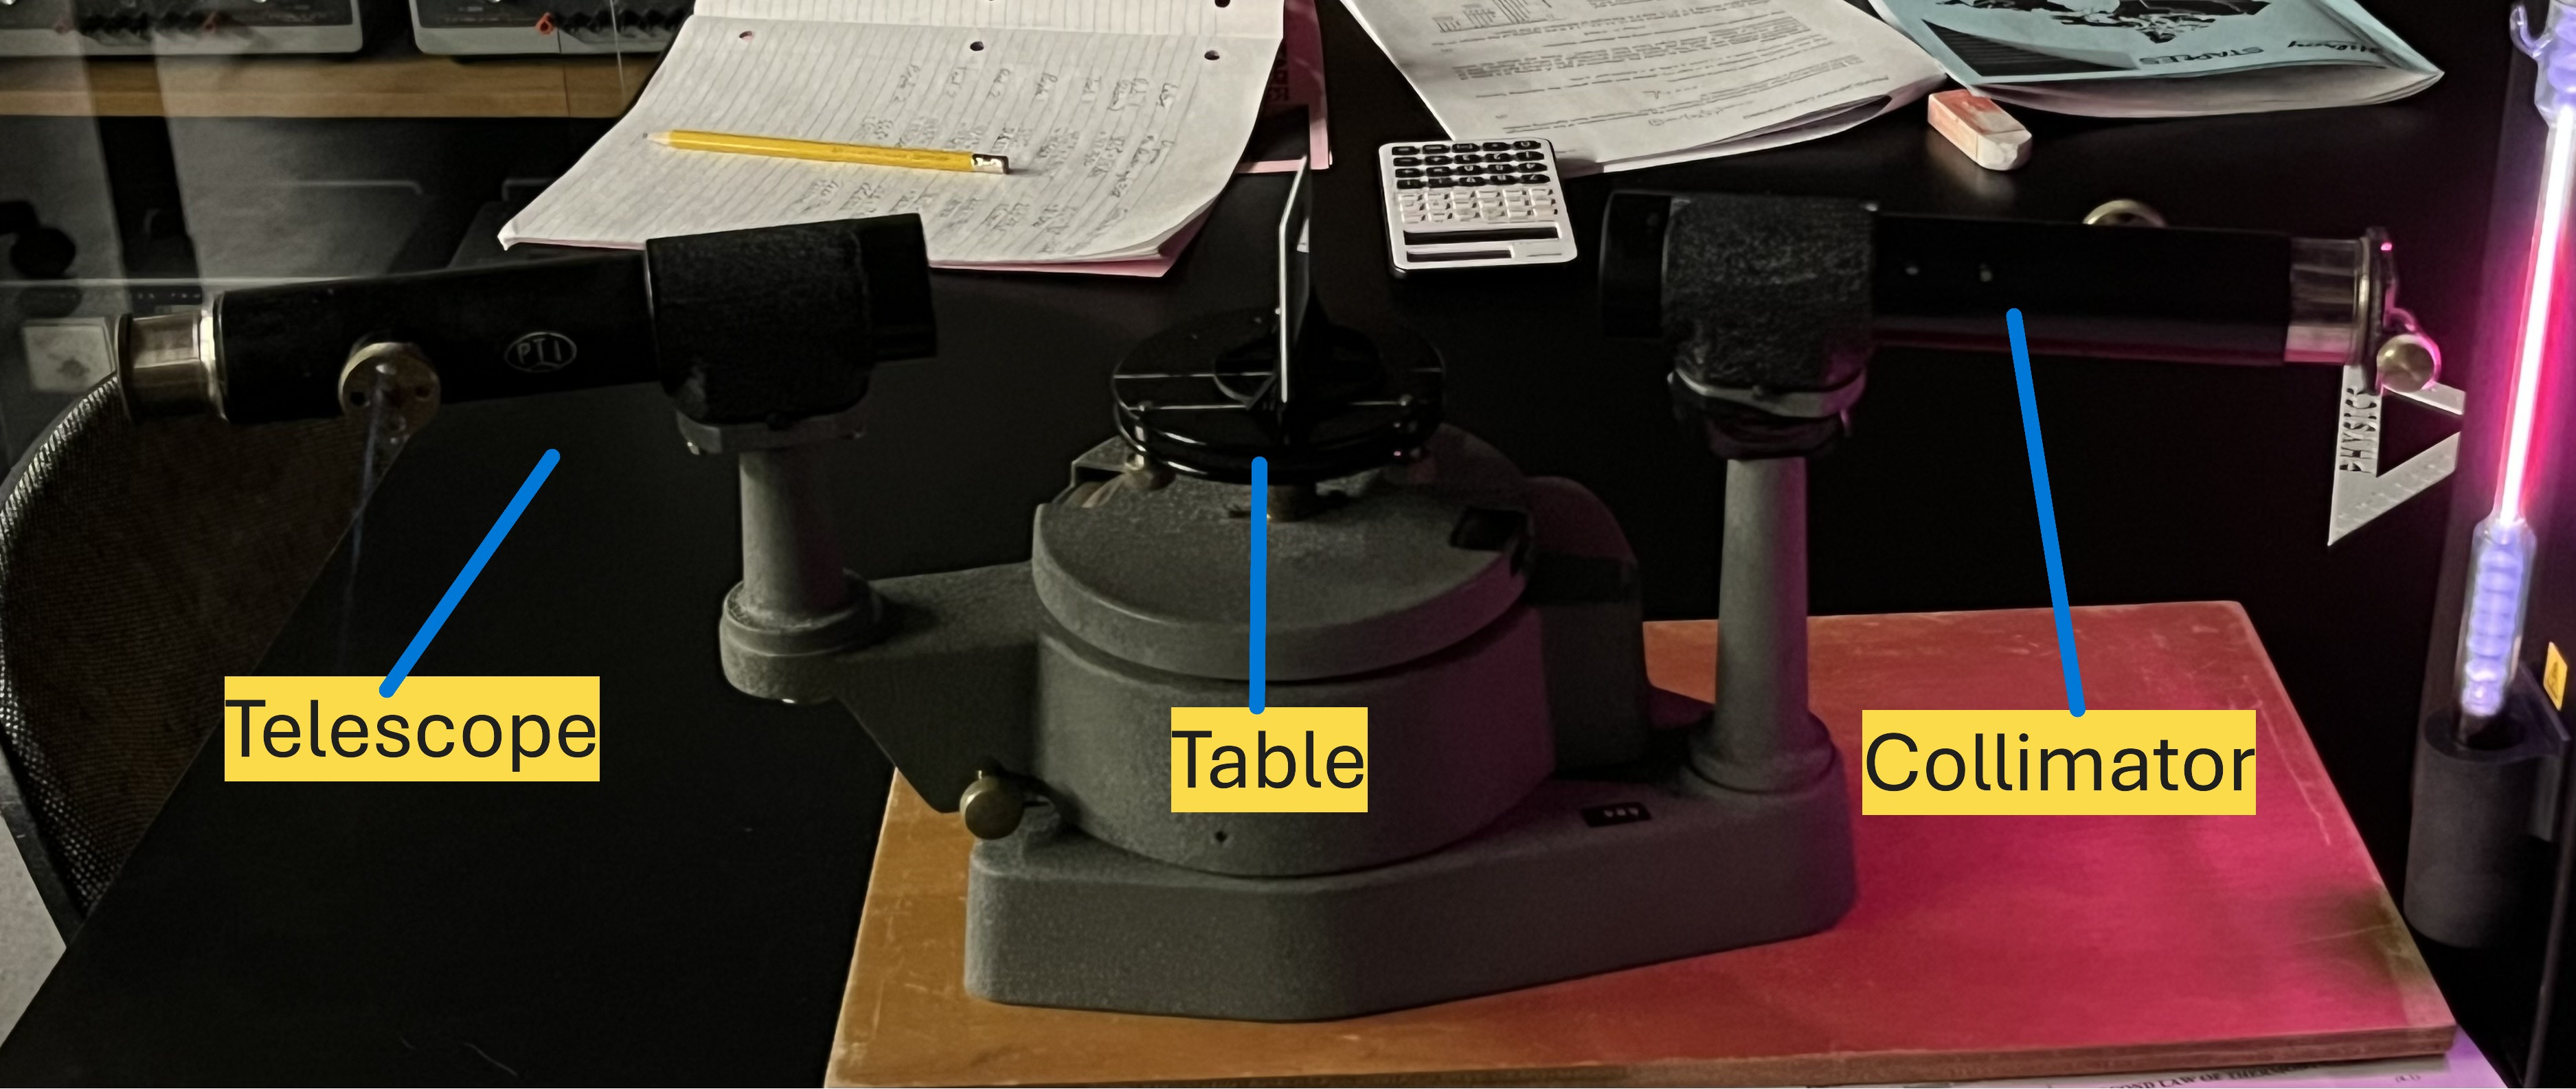
\includegraphics[width=0.8\columnwidth]{H-Spectrum Lab photos/Spectrometer_Markup.JPG}
        \caption{\label{fig1}A desktop spectrometer. Light enters the collimator from the hydrogen lamp [right] and focuses toward the table. A diffraction device is placed on the table, and the telescope and table are adjusted as needed to view the spectral emissions. 
        }
\end{figure}

\begin{figure}[H] 
        \centering 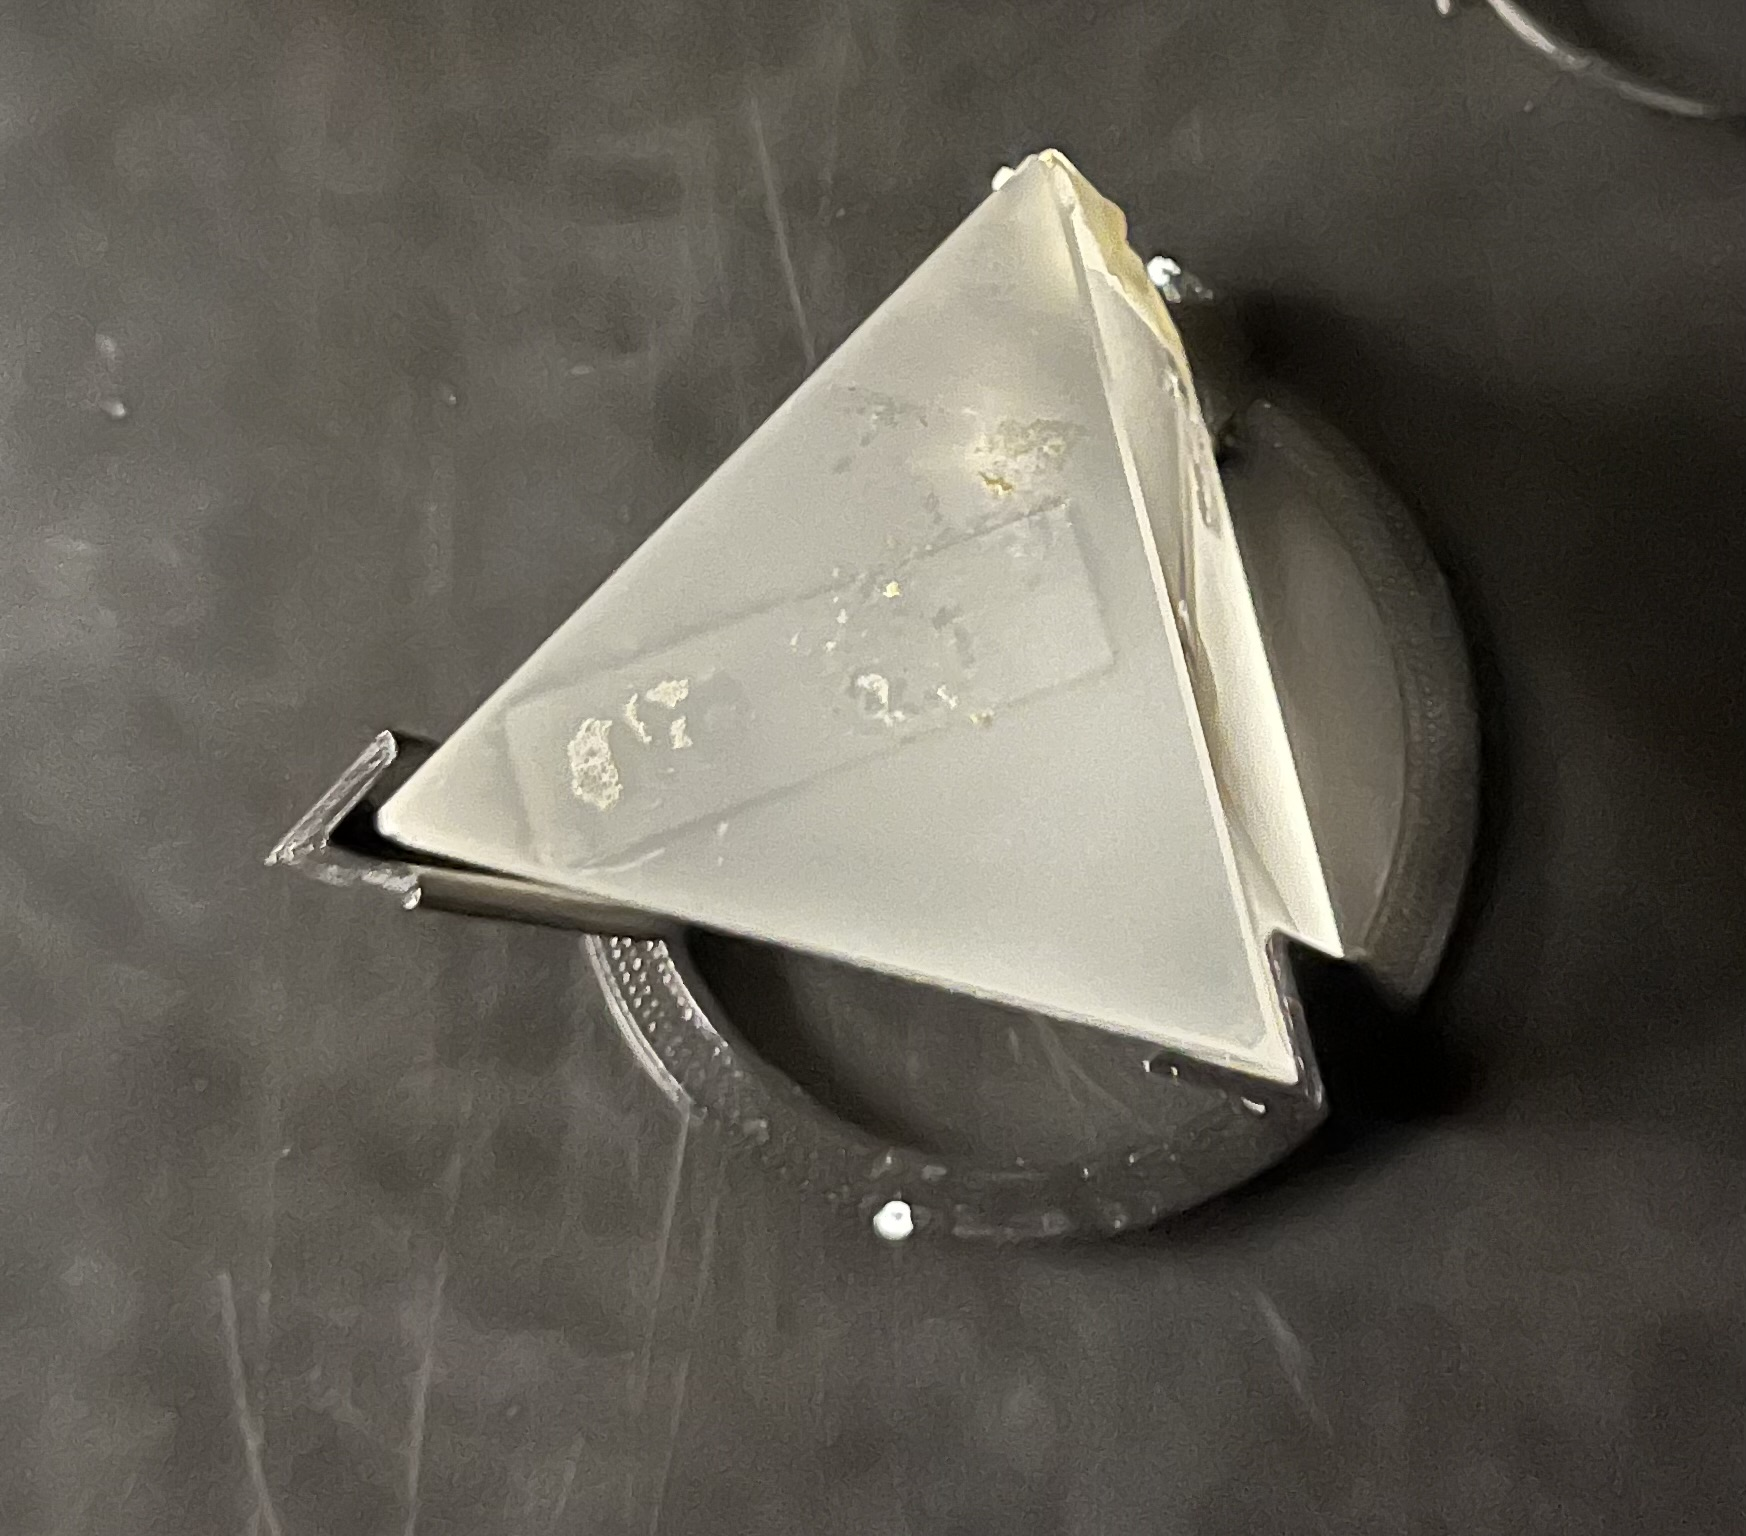
\includegraphics[width=0.4\columnwidth, height=6\headheight]{H-Spectrum Lab photos/Prism.jpg}
        \centering 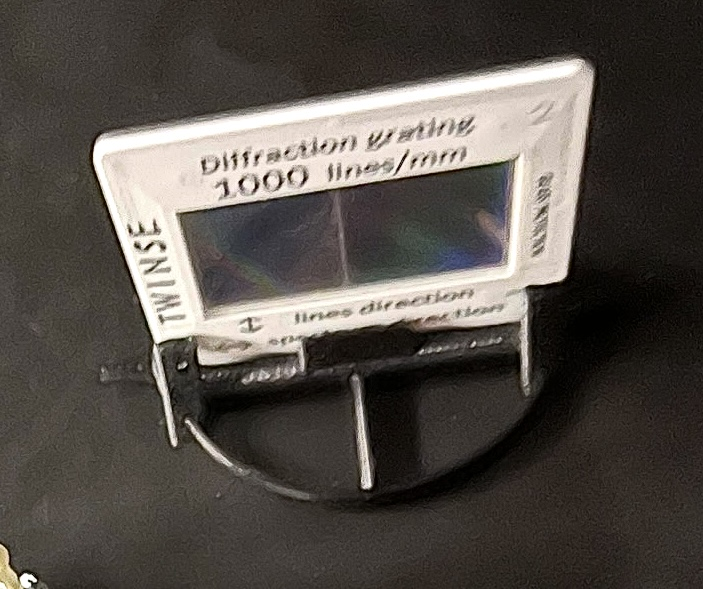
\includegraphics[width=0.4\columnwidth, height=6\headheight]{H-Spectrum Lab photos/Grating.jpg}
         \caption{\label{fig5}Diffraction Devices, Prism [left] and Diffraction Grating [right].}
\end{figure}



\subsection{Method: Using the prism}

 The lab began by placing the hydrogen lamp (Fig. \ref{fig2}) directly in front of the collimator and turning it on. The prism was then placed on the table of the spectrometer with the incident angle $<$ 90\textdegree\text{} (Fig. \ref{fig3}). The telescope was then rotated counterclockwise trying to locate the spectral lines. It wasn’t long until the first wavelength, that of red light ($\approx$ 650 nm), appeared in the telescope. Having located the light emission, the table was rotated slightly back and forth until the point of minimum deviation was reached. The point of minimum deviation was the point when the rotation of the table in either direction resulted in the rightward movement of the light in the telescope. No matter what direction the table was turned, the light could not be refracted further left. After lining up the crosshair of the telescope on the right-hand side of the wavelength (Fig. \ref{fig4}), the first measurements were taken using the vernier\footnote{The vernier scale is built directly into the spectrometer, and allows users to accurately measure the angle up to 2 decimal places} scale. This process then occurred for the other spectral lines and was repeated once so that secondary data was collected.  


\begin{figure}[H] 
        \centering 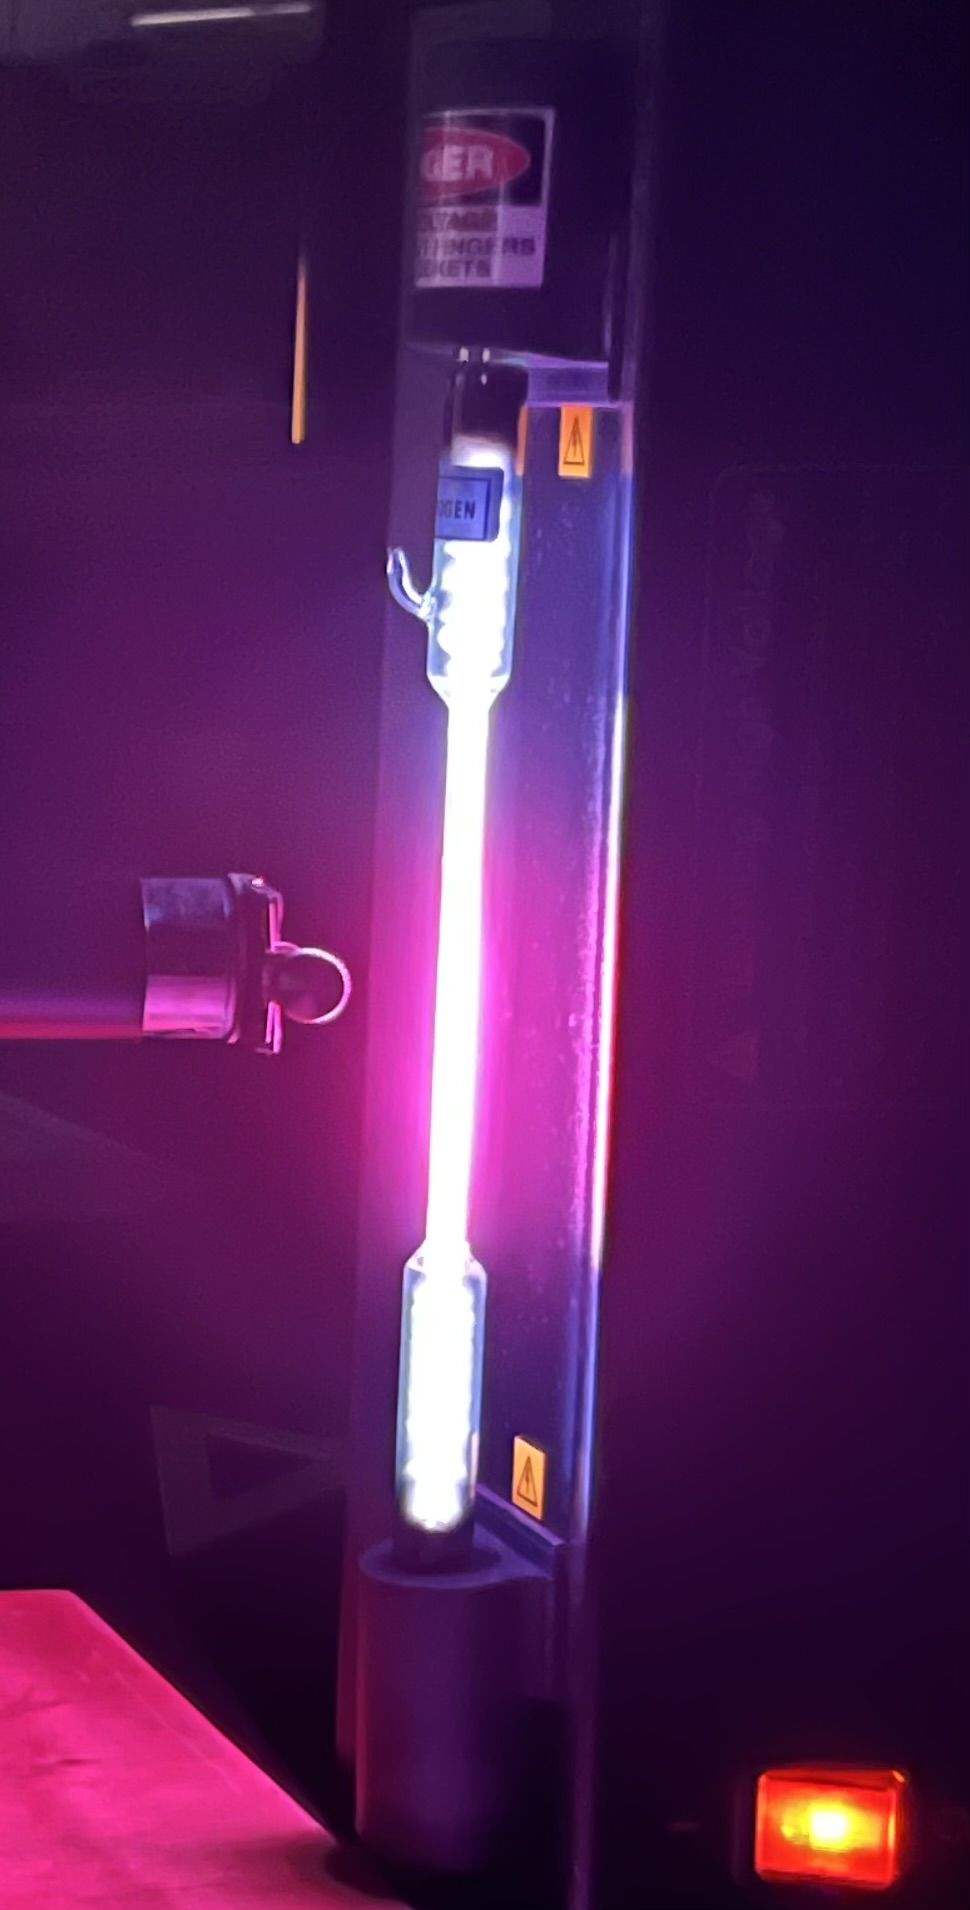
\includegraphics[width=0.7\columnwidth, height=10\headheight]{H-Spectrum Lab photos/H-lamp.jpg}
        \caption{\label{fig2}Hydrogen Lamp. It emits light given off by electrons falling down energy levels in individual atoms.
        }
\end{figure}


 \begin{figure}[H] 
        \centering 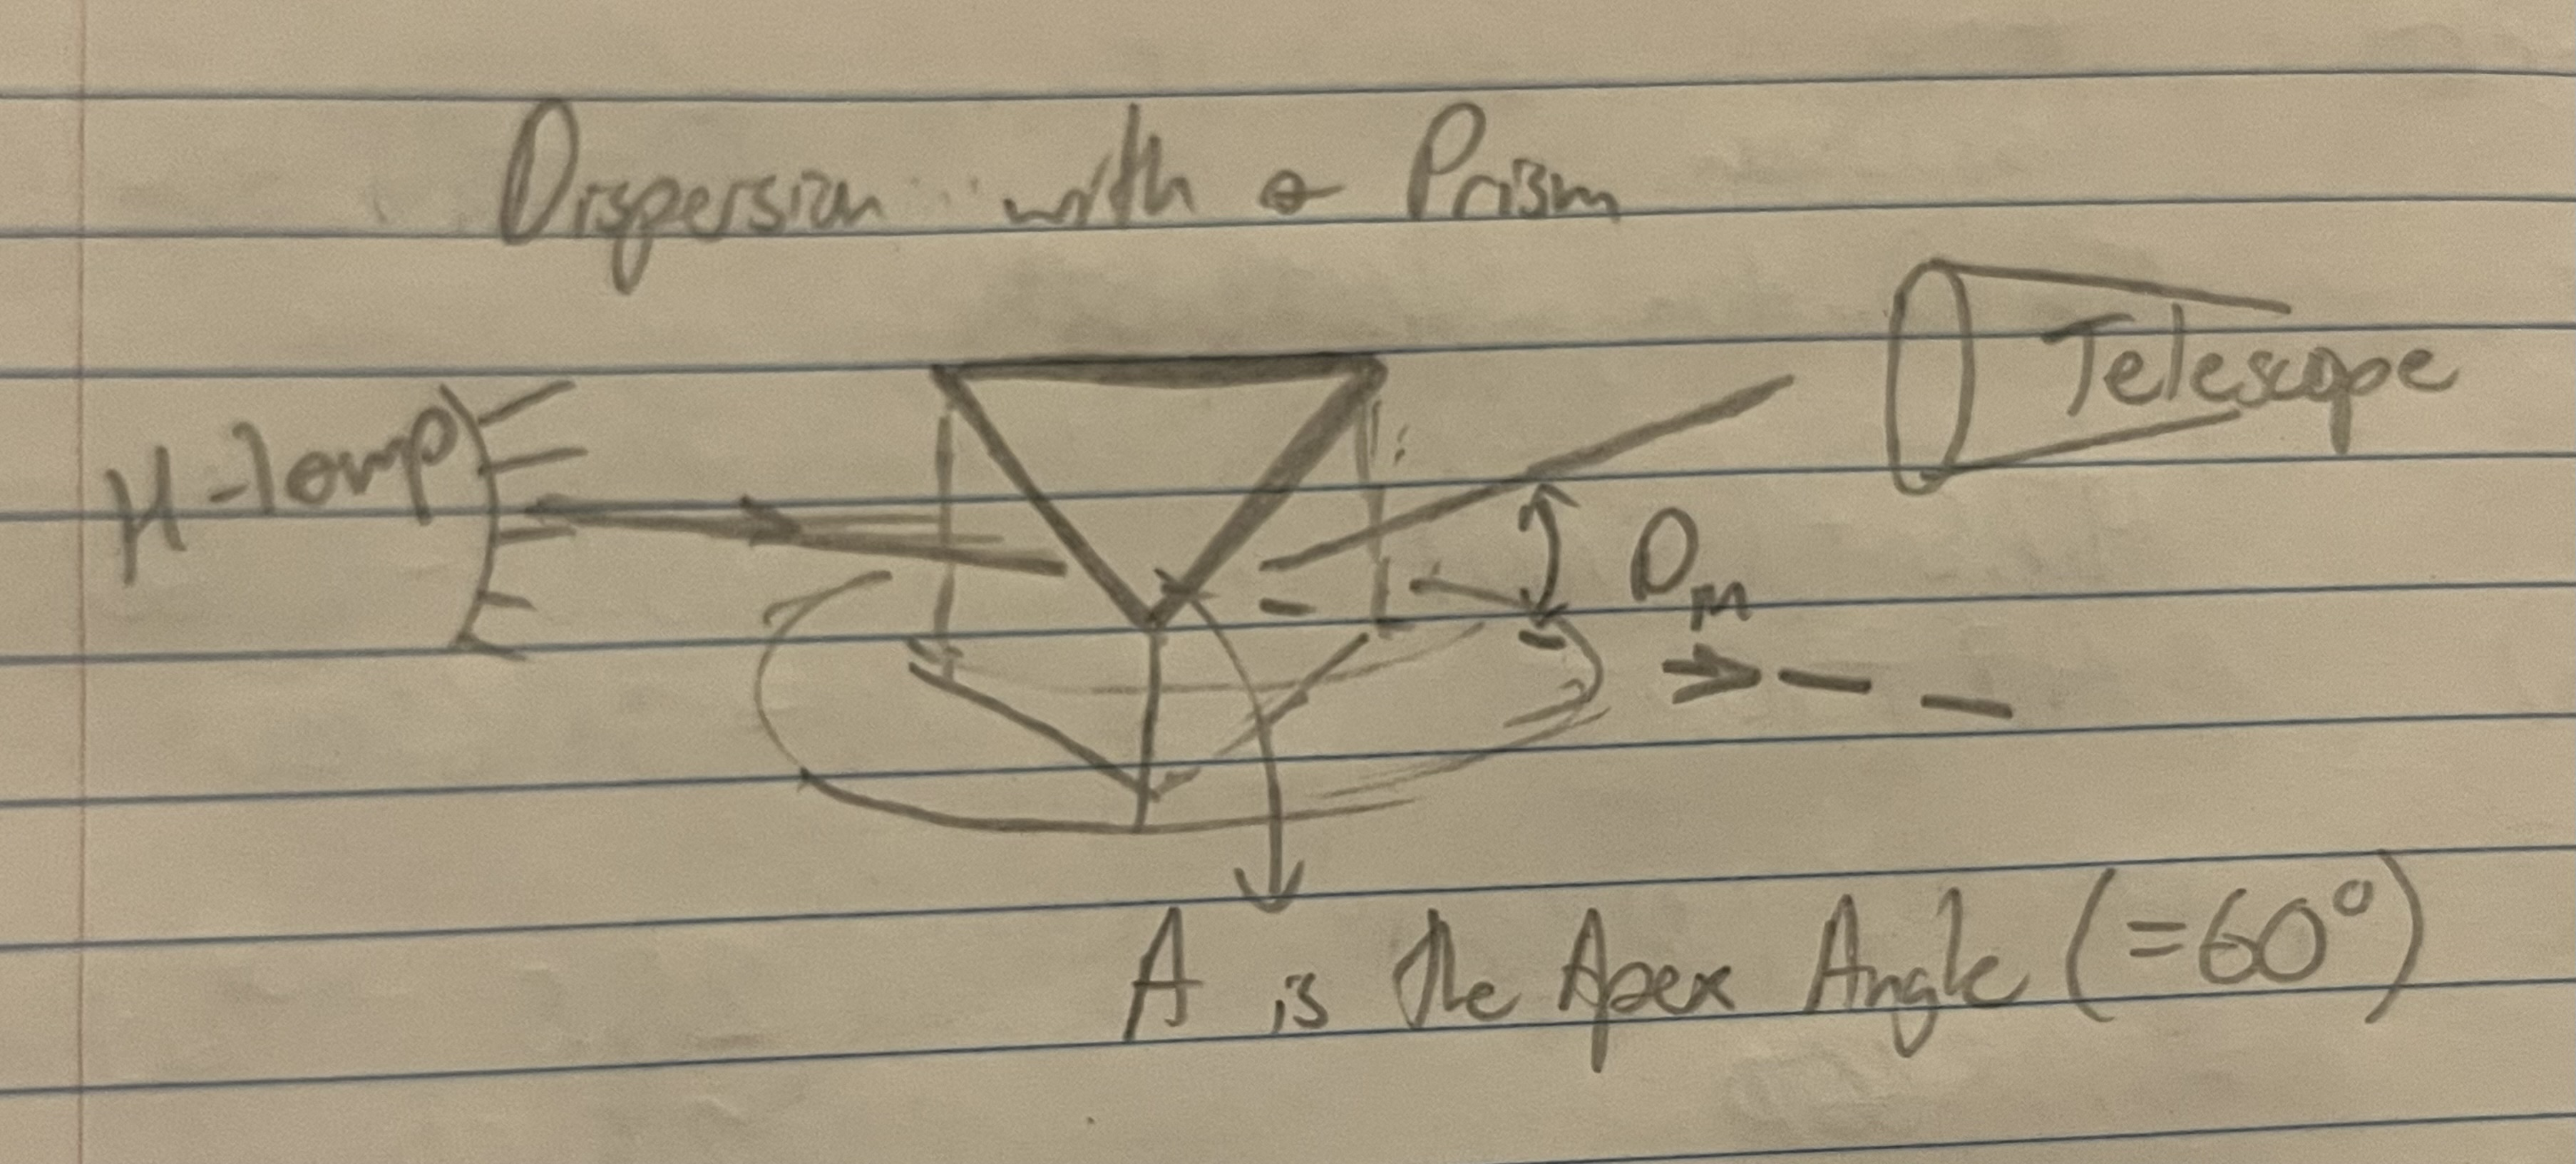
\includegraphics[width=0.8\columnwidth]{H-Spectrum Lab photos/Prism Drawing.jpg}
        \caption{\label{fig3}A labeled diagram showing the angles involved in measuring light dispersing through a prism.
        }
\end{figure}

\subsection{Method: Using the Diffraction Grating}

Similarly to the prism, this process began by placing the diffraction grating on the table. However, instead of the incident angle being $<$ 90\textdegree\text{}, it needs to be $=$ 90\textdegree\text{}. This is because the dispersion angle needs to be measured from the original incident beam. If the diffraction grating is askew, the measured angle will be proportionally askew, and the corresponding wavelength values will exhibit systemic error. However, without any special tools to assist in placing the diffraction grating as precisely as possible, this must be expected in the results. Once the grating had been placed in a reasonable location, the spectral lines in the telescope (Fig. \ref{fig4}) must once again be found. It was more difficult in this experiment as the spectral lines were very dim. Despite this, they were successfully located and the appropriate measurements were made. 

\begin{figure}[H] 
        \centering 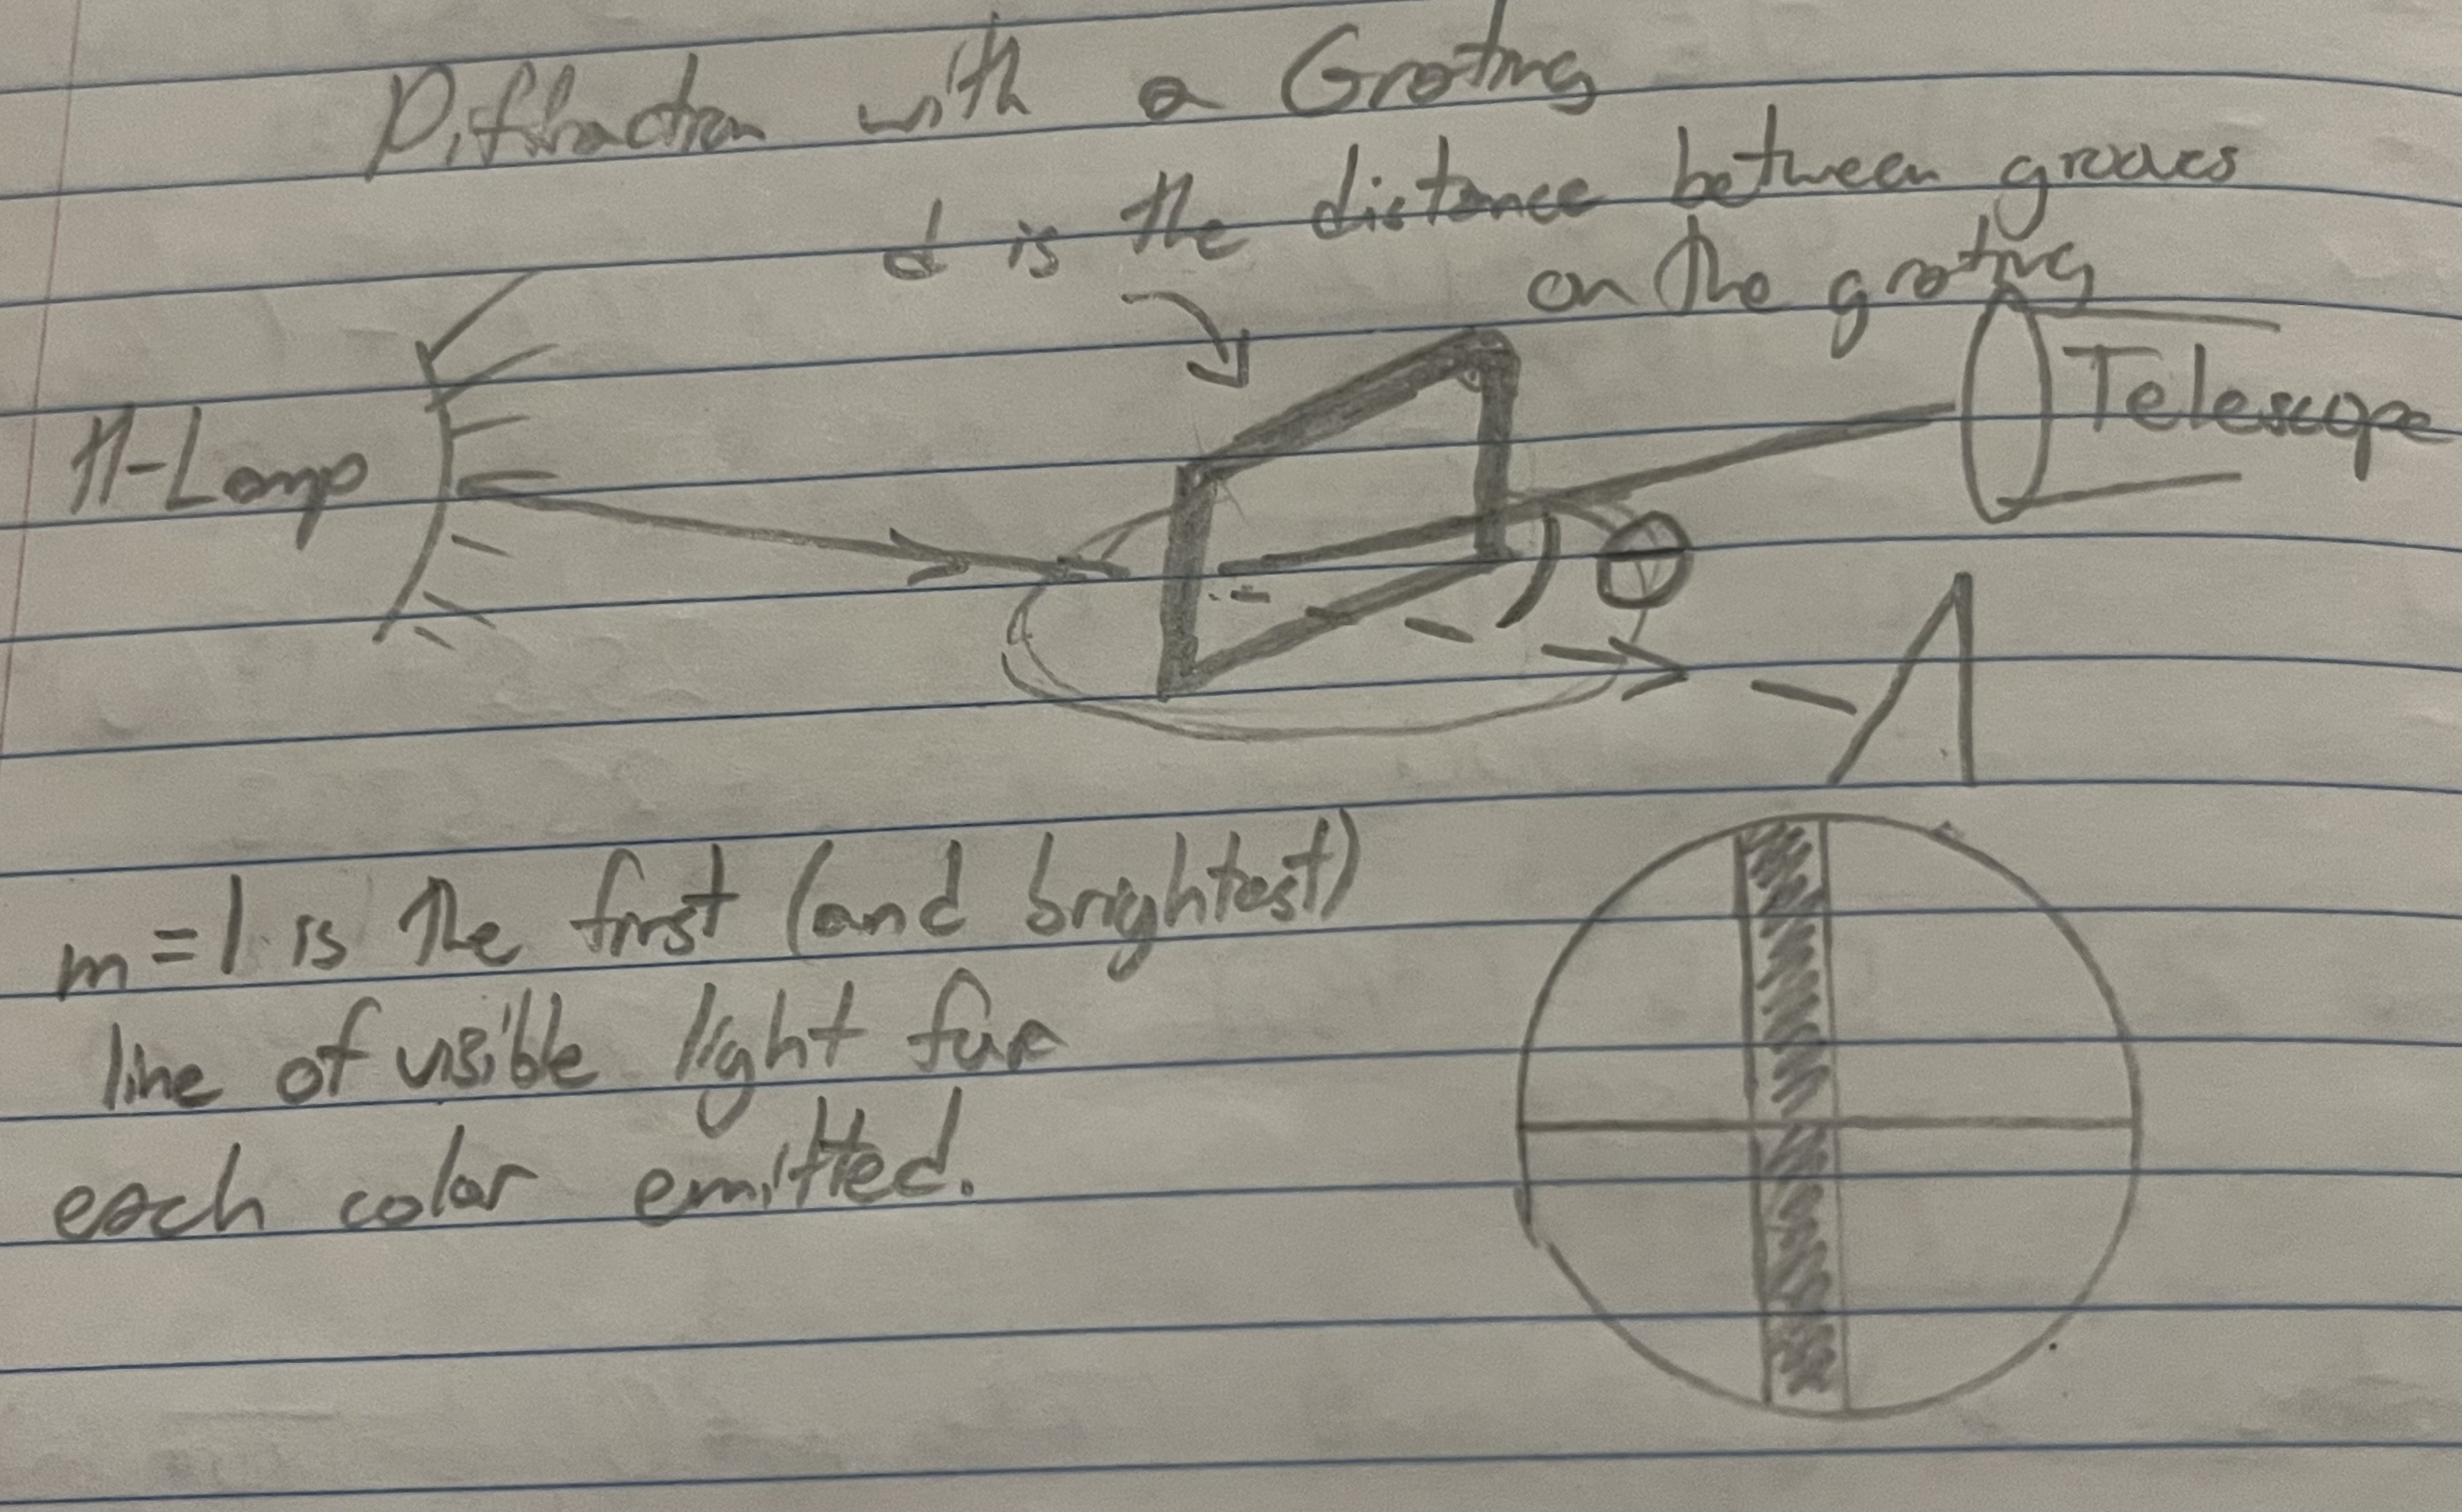
\includegraphics[width=0.8\columnwidth]{H-Spectrum Lab photos/Diffraction Grating Drawing.jpg}
        \caption{\label{fig4}The use of a diffraction grating and spectrometer to locate spectral lines.
        }
\end{figure}

\section{Results and Analysis}

\subsection{Observations: The Prism}

The prism was initially difficult to use as it requires some time and effort to place it correctly. Once we did so, it didn't take long to identify when the wavelengths of light were at their minimum deviation.

\begin{table}[h]
    \centering
    \caption{Comparing known theoretical wavelengths of hydrogen's visible emission spectrum, to calculated wavelengths computed through the measurement of a corresponding angle. The angle was generated by an equilateral prism, and was examined through a desktop spectrometer telescope.}
    \label{tab:prism data} 
    
    % IN THIS TABLE UNCERTAINTY IS EITHER 0.08 OR 0.1 FOR THE %CALCULATED WAVELENGTH

    \begin{tabular}{|c|c|c|c|c|}
        \hline
        Color & Theo. Wavelength  & Min. Deviation Angle  & Calc. Wavelength & \% Diff. \\
        \hspace{0 pt}
          & ($\lambda_{theo.}$) (nm) & ($D_M$) $\pm 0.02$(\textdegree) & ($\lambda_{disp.}$) $\pm 5\%$(nm) & \\
        \hline
        \hline
        Red    &656.34 & 47.75 & 650.69    & 0.9   \\
        \hline
        Red    &656.34 & 47.78 & 646.16   & 1.6  \\
        \hline
        Teal   & 486.17   &  49.57 & 479.27   &  1.4  \\
        \hline
        Teal   & 486.17  &  49.50  & 483.50   & 0.6     \\
        \hline
        Purple    & 434.08  & 51.68  & 389.09&  10.4  \\
        \hline
        Purple  &  434.08 &  50.55  & 430.03 & 0.9     \\
        \hline 
    \end{tabular}
\end{table}

This half of the lab was very accurate, with the data in Table \ref{tab:prism data} giving results within the 5\% uncertainty range. In fact, the majority of the measurements are within 2\% of the expected value\footnote{2\% of the theoretical wavelengths are 1. [red] 13.13nm 2. [teal] 9.72nm and 3. [purple] 8.68nm}. The one exception to this is the initial measurement of purple with $\lambda_{disp.}=389.09\pm19.453$nm. This value is an anomaly and is likely the result of a erroneous measurement, or movement of equipment. This would mean that the angle of minimum deviation was \underline{not} measured, but rather some other in-accurate angle was recorded. 

However, the general accuracy between the theoretical wavelength and calculated wavelength, most obvious in the \% difference, supports the idea of quantized energy levels obeying equations \ref{eq1} and \ref{eq4}.

\subsection{Observations: The Diffraction Grating}

Placing the diffraction grating was by far the most error prone part of this lab. With no way to ensure precision in lining it up perfectly perpendicular to the collimator, some systematic error in our measurements was expected.

\begin{table}[h]
    \centering
    \caption{Comparing theoretical wavelengths of the light spectrum emitted by excited hydrogen particles to values calculated from measured diffraction angles. The light was diffracted using a grating with spacings $1\times10^{-6}$m apart.}
    \label{tab:grating data}
    \begin{tabular}{|c|c|c|c|c|}
        \hline
        Color & Theo. Wavelength
        & Diffraction Angle  & Calc. Wavelength  & \% Diff. \\
        \hspace{0 pt}
           & ($\lambda_{theo.}$) (nm) & ($\theta$) $\pm 0.02$(\textdegree) & ($\lambda_{diff.}$) $\pm0.3$(nm) &  \\
        \hline
        \hline
        Red    &656.34 & 35.65 & 582.83  & 11.2    \\
        \hline
        Red    &656.34    &  36.32&592.25 &  9.8        \\
        \hline
        Teal   & 486.17 & 25.50  &  430.51 &   11.4       \\
        \hline
        Teal   & 486.17  & 25.63 &432.61 & 11.0       \\
        \hline
        Purple & 434.08 & 22.58& 384.03    & 11.5         \\
        \hline
        Purple &   434.08 &  22.50 &382.68  & 11.8       \\
        \hline
    \end{tabular}
\end{table}

 This is exactly what we get in Table \ref{tab:grating data}. The leftmost column has 5 values\footnote{With the lone exception being the secondary measurement of the red wavelength. This is likely a result of incorrectly placing the crosshair, or potentially moving the diffraction grating or spectrometer.} that are $\approx 11\%$ different then the theoretical value. This is the definition of systematic error. Although it might not have been apparent while conducting the experiment, the diffraction grating was most certainly askew. 

Furthermore, when considering the high accuracy of the vernier scale, $\pm 0.02$\textdegree\text{}, the error in the measurements is very low. The systematic error is only evident in the \% difference. Even considering the uncertainty range the calculated wavelengths are much too small to be accurate. An example of this is the first measurement of the red wavelength. With a value of $\lambda_{diff.}=582.83$nm the human eye should perceive green light. This was not the case, and so we know this is the result of systematic error. 

A quick way to check this would be to find the theoretical angle $\theta$ corresponding with the theoretical $\lambda$ value. The calculation can be seen in section \ref{calc}, but its result is interesting. For $\lambda_{theo.} = 656.34$nm we have a $\theta_{theo.}=41.02$\textdegree\text{}. This would imply that our diffraction grating was askew by an angle of $\approx5$\textdegree\text{} as can be seen by the angle analysis in Fig. \ref{askew}.

\begin{figure}[H]
        \centering 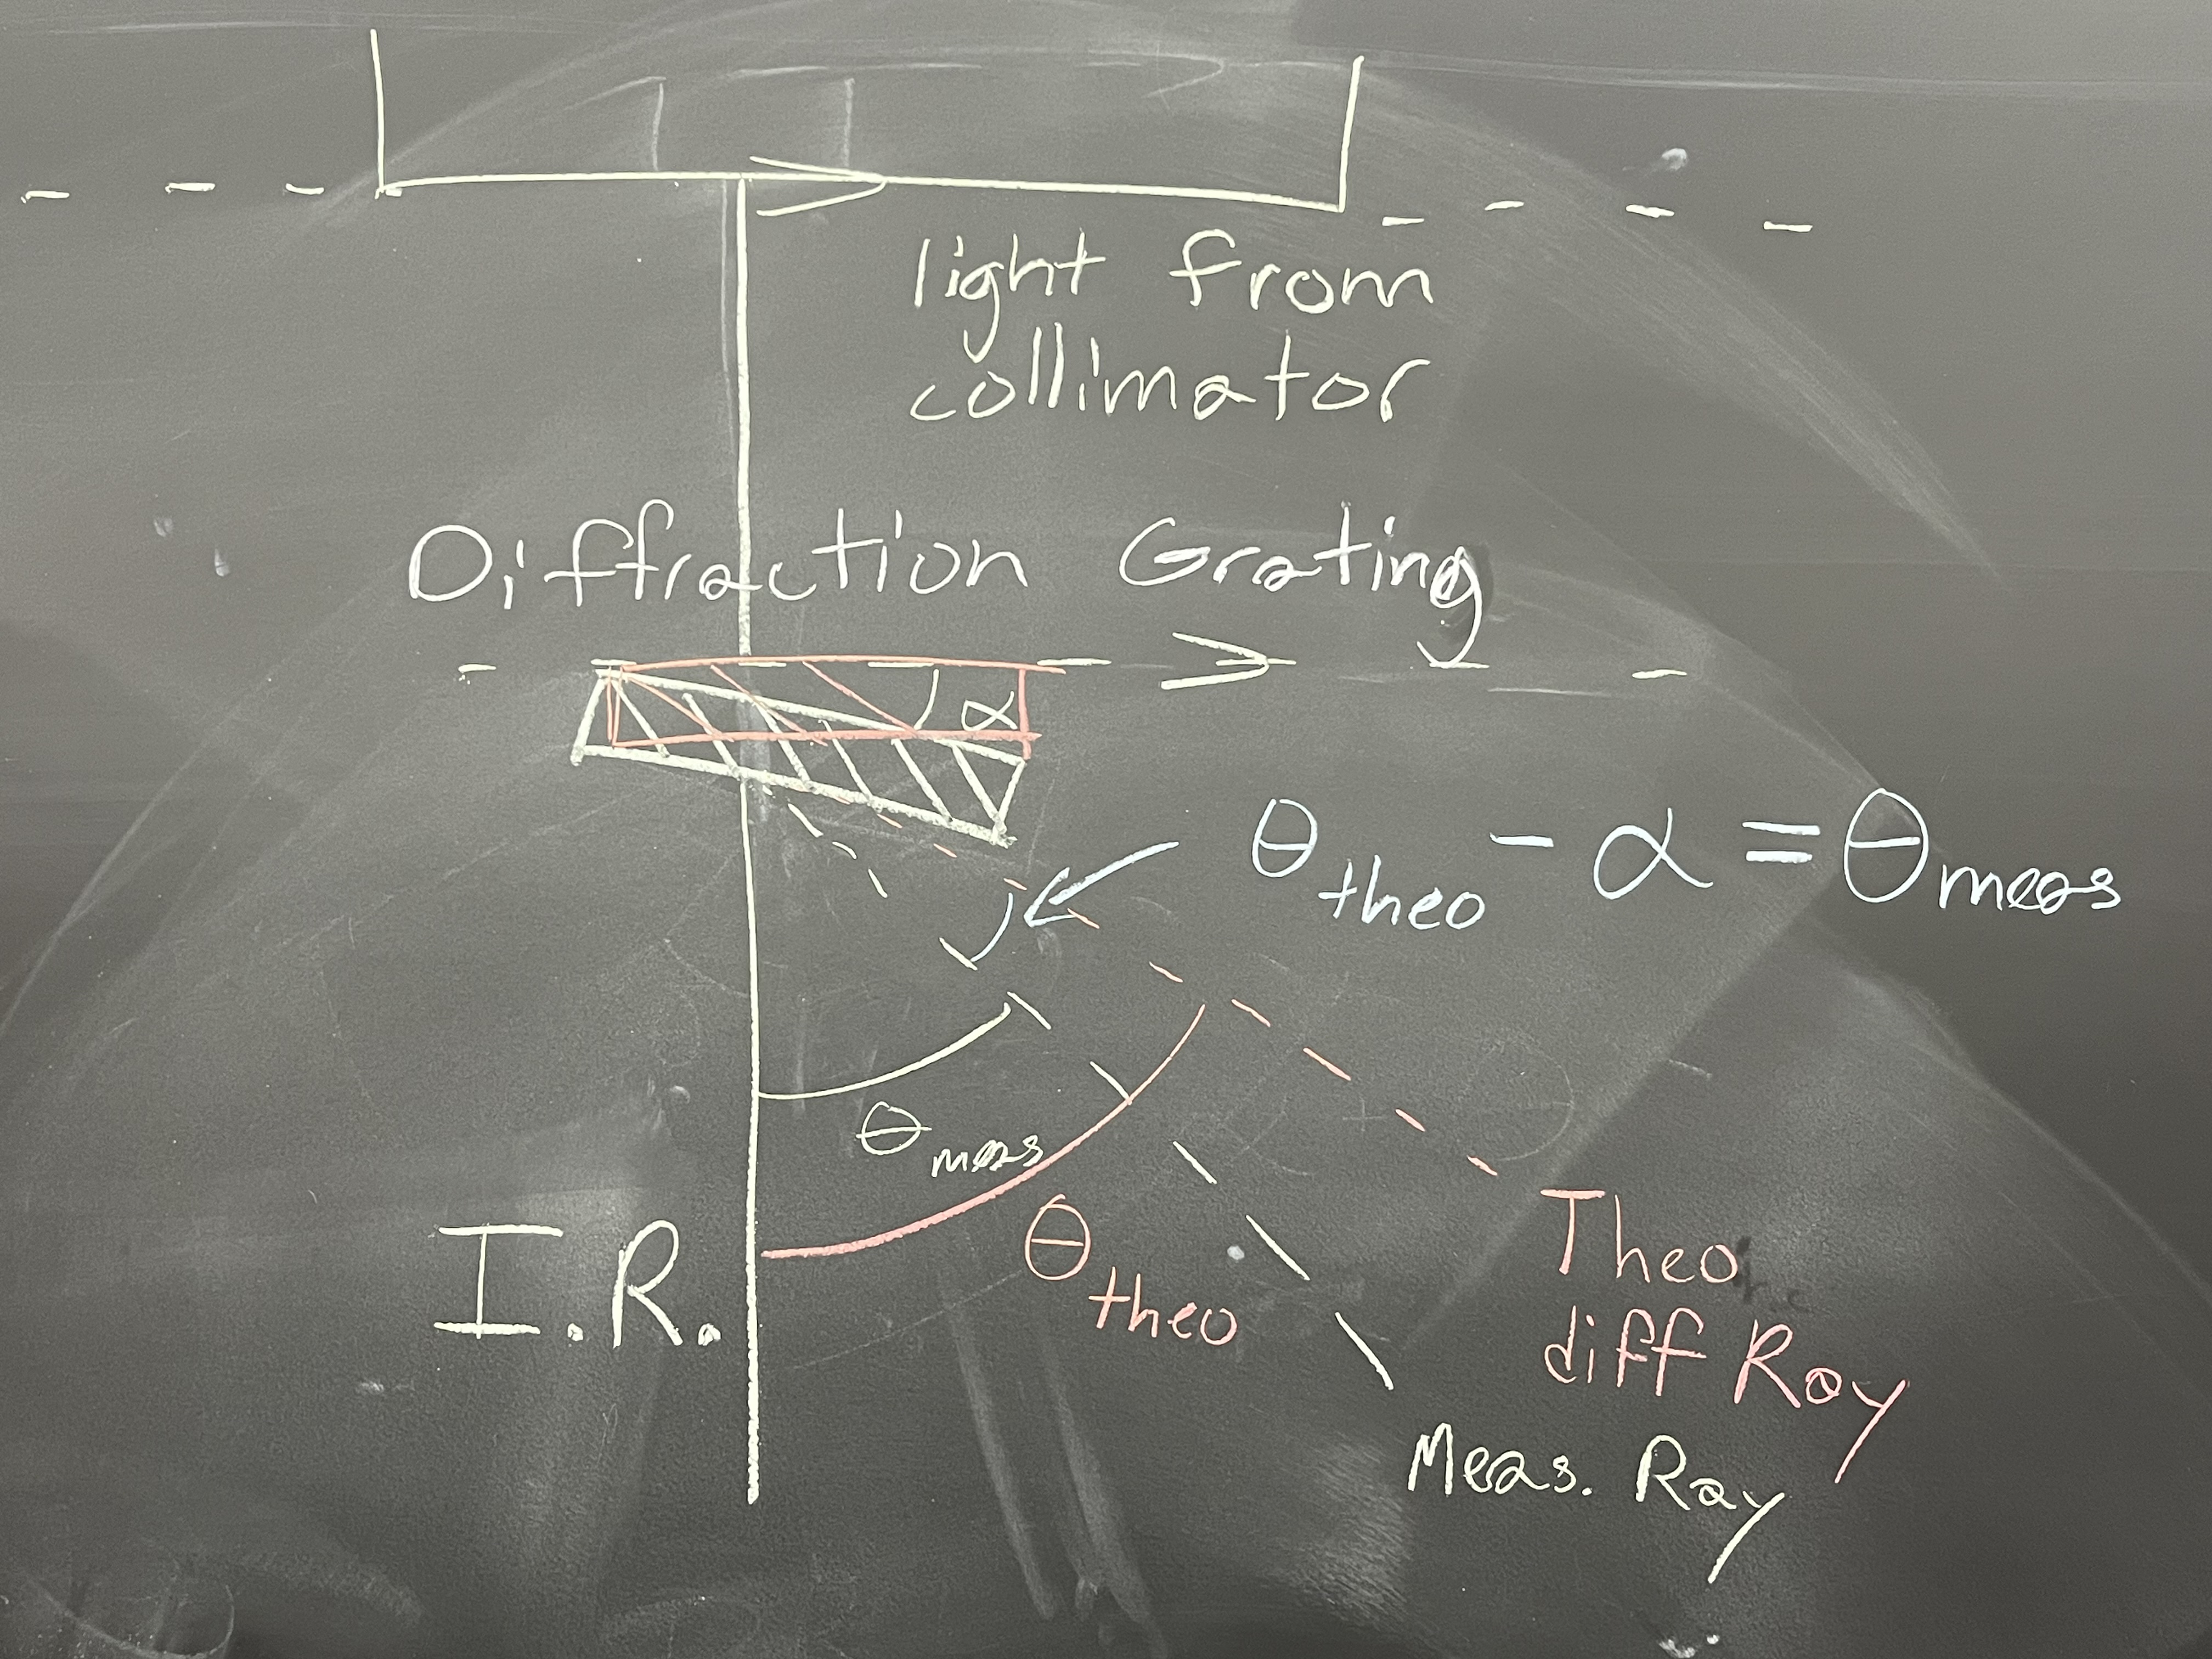
\includegraphics[width=0.8\columnwidth]{H-Spectrum Lab photos/IMG_0701.jpg}
        \caption{\label{askew}Analyzing the use of the diffraction grating in the lab.
        }
\end{figure}


\subsection{Sources of Error}

The instruments used in this lab are very precise pieces of equipment, with little reason to believe they could cause error. However, as is the case with any lab, small uncertainties in many parts of the lab may add up and contribute to overall lab error. 

\textbf{The Telescope:}
The telescope had several knobs which could be used to fine tune and focus the instrument. Despite this, the crosshair never evenly lined up with the entire line spectral. It often seemed to bend into the light at the top and bottom. This is likely an effect of the equipment (or tables) not being perfectly level and thus creating the unintended curving. The effect of this on the experiments results is likely minimal, but still worth noting if this experiment were to be performed again.

\textbf{Hydrogen Lamp:}
The hydrogen lamp runs on a large amount of electricity, which is necessary to provide the energy to move electrons in the atoms. Error could appear through fluctuations in the amount of energy supplied, causing the measured wavelengths edges to become dim. As a result of this, the crosshair may not have truly been at the edge of the line spectral, causing less precise measurements.

\textbf{Diffraction Devices:}
Both diffraction devices have the opportunity for error to appear. For instance, either device could have a smudge or blemish on it which changes the angle of diffraction and thus the recorded measurement.

When you consider all of these things at once, it becomes apparent that no lab will be perfect. Despite this, the majority of the results in Tables \ref{tab:prism data} and \ref{tab:grating data} are close to theoretical values, or off by some explainable systematic error, and thus justifiably accurate. 

\subsection{Potential Improvements}
If this lab were to be conducted again I would highly suggest finding a solution to the diffraction grating orientation problem. Using a perfectly square object or other method (such as effectively measuring the askew angle of the diffraction gratings placement) to ensure as little systematic error as possible enters into the collected data. Beyond that, one could attempt to take many measurements of the minimum deviation angle, and adjust the table (or prism) each time to allow for a mean value (and corresponding uncertainty) to be reported. This could reduce the deviation appearing when just two data points are collected.

\section{Conclusion}

It was the purpose of this lab to show whether or not Bohr's theory of quantized energy levels in atoms was based on factual evidence. For his theory to be considered correct, it must be that excited atoms only release wavelengths corresponding to their energy levels. As was demonstrated through the use of a prism and diffraction grating, we saw Bohr's theory is indeed correct. Only specific wavelengths were seen diffracted, and the measured angles corresponded nicely. Take for example the teal line spectrum seen through the prism. The measured value of $483.50 \pm0.04\%$nm is quite close to the theoretical value of $486.17$nm. In fact it is a mere $0.6\%$ different, well within the uncertainty of $\pm5\%$ (Table \ref{tab:prism data}). This relative error is small enough to explain by uncontrollable factors in the lab equipment and environment. As a result, the lab achieved its goal to test Bohr's theory, and found that electrons do indeed exist at quantized energy levels as he predicted long ago.

\clearpage
\appendix
\section{Appendix} \label{append}

\subsection{Deriving Formulas}

Equating Equations \ref{eq2} and \ref{eq3}:


\begin{DispWithArrows*}
    1.5935 + \frac{0.0093\times 10^{-12}}{\lambda_{dispersion}^2} &= \frac{\sin(\frac{A + D_M}{2})}{\sin(\frac{A}{2})} \\
    \frac{0.0093\times 10^{-12}}{\lambda_{dispersion}^2} &= 
    \frac{\sin(\frac{A + D_M}{2})}{\sin(\frac{A}{2})} - 1.5935 \\
    \frac{\lambda_{dispersion}^2}{0.0093\times 10^{-12}} &=
    \frac{1}{\frac{\sin(\frac{A + D_M}{2})}{\sin(\frac{A}{2})} - 1.5935} \\
    \lambda_{dispersion}^2 &= \frac{0.0093\times 10^{-12}}{\frac{\sin(\frac{A + D_M}{2})}{\sin(\frac{A}{2})} - 1.5935} \\
    \lambda_{dispersion} &= \sqrt{\frac{0.0093\times 10^{-12}}{\frac{\sin(\frac{A + D_M}{2})}{\sin(\frac{A}{2})} - 1.5935}} \\
    \lambda_{dispersion} &= \sqrt{\frac{0.0093\times 10^{-12}}{2\sin\left(30+\frac{D_M}{2}\right) - 1.5935}} \qedhere
\end{DispWithArrows*}


\subsection{Sample Calculations}

Calculating Percent Difference: Taking $\lambda_{theo.}= 656.34\text{nm}$ and  $\lambda_{meas.} = 650.69\text{nm}$ from Table \ref{tab:prism data}.
\begin{DispWithArrows*}
    \% \text{ Difference} &= \lvert \frac{\lambda_{meas.} - \lambda_{theo.}}{\lambda_{theo.}} \rvert \times 100\%\\
    &= \lvert\frac{650.69 - 656.34}{656.34}\rvert \times 100\%\\
    &= \lvert-0.00860834\rvert \times 100\% \\ 
    &= 0.00860834 \times 100\% \\ 
    &= 0.9\%\qedhere
\end{DispWithArrows*}



Calculating $\lambda_{disp.} = \sqrt{\frac{0.0093\times 10^{-12}}{2\sin\left(30+\frac{D_M}{2}\right) - 1.5935}}$ using $D_M = 47.75$\textdegree\text{} from Table \ref{tab:prism data}.
\begin{DispWithArrows*}
    \lambda_{disp.} &= \sqrt{\frac{0.0093\times 10^{-12}}{2\sin\left(30+\frac{D_M}{2}\right) - 1.5935}} \\
    &=  \sqrt{\frac{0.0093\times 10^{-12}}{2\sin\left(30+\frac{47.75}{2}\right) - 1.5935}} \\
    &= 6.506860 \times 10^(-7) \text{m} \\
    &= 650.6860 \text{nm}\\
    &= 650.69\text{nm}\qedhere
\end{DispWithArrows*}

Calculating $m\lambda_{diff.} = d \sin(\theta)$ using $m=1$ and $\theta = 35.65$\textdegree\text{} from Table \ref{tab:grating data}.

\begin{DispWithArrows*}
    m\lambda_{diff.} &= d \sin(\theta) \\
    &= \frac{(1\times10^{-6})\sin(35.65)}{1}        \\
    &= 5.828323 \times 10^(-7) \text{m} \\
    &= 582.8323 \text{nm}\\
    &= 582.83\text{nm}\qedhere
\end{DispWithArrows*}

Calculating Error Propagation of Uncertainty for $\lambda_{diff.}$:
\begin{DispWithArrows*}
    \delta\lambda_{diff.} &= \sqrt{(\frac{\partial\lambda}{\partial{d}}\partial{d})^2 + (\frac{\partial\lambda}{\partial\theta}\partial\theta)^2} \\
    &= \sqrt{(\sin(\theta)\partial{d})^2 + (d\cos(\theta)\partial\theta)^2} \\
    &= \sqrt{(\sin(\theta)(0)^2 + (d\cos(\theta)(0.02 \times\frac{\pi}{180})^2} \\
    &= \sqrt{((1\times 10^{-6})\cos(0.02 \times\frac{\pi}{180})(0.02 \times\frac{\pi}{180})^2} \\
    &= 3.49065 \times 10^{-10}\text{m} \\
    &= 0.349065\text{nm} \\
    &= 0.3\text{nm} \qedhere
\end{DispWithArrows*}

Calculating Uncertainty, $\delta\lambda_{disp.}$, using $D_M = 47.75$\textdegree\text{} and associated uncertainty $\delta D_M =0.02$\textdegree\text{}.

\begin{DispWithArrows*}
    \frac{\delta\lambda_{disp.}}{\lambda_{disp.}} &= \frac{\delta D_M}{D_M} \times 100\%\\
    &= \frac{\delta D_M}{D_M}\lambda_{disp.}\times 100\% \\
    &= \left(\frac{0.02}{47.75}\right)\lambda_{disp.} \times 100\% \\
    &=0.00041885\lambda_{disp.} \times 100\% \\
    &=0.04\% \times \lambda_{disp.} \qedhere
\end{DispWithArrows*}

As the uncertainty value of $\beta$ (5\%)is the largest of the three variables in our expression for $\lambda_{disp}$ we can approximate by: 
\begin{DispWithArrows*}
    \frac{\delta\lambda_{disp.}}{\lambda_{disp.}} &\approx \sqrt{(\frac{\partial D_M}{D_M})^2 + (\frac{\partial\alpha}{\alpha})^2 + (\frac{\partial\beta}{\beta})^2} \\
    &\approx \sqrt{(\frac{\partial\beta}{\beta})^2} \\
    &\approx \frac{\partial\beta}{\beta} \\
    &\approx 5\%* \qedhere
\end{DispWithArrows*}
*This is the value used in Table \ref{tab:prism data}.

\newpage

\subsection{Raw Data}

\begin{table}[ht]
    \centering
    \begin{tabular}{|c|c|c|c|}
    \hline
        Color (Test Number) & Deviation Angle (\textdegree)& Minutes ($'$) & Total Angle (\textdegree)\\
        \hline
        Red (1) & 47.5 & 15 &  47.75 \\
        \hline
        Red (2) & 47.5 & 17 & 47.78\\
        \hline
        Teal (1) & 49.5 & 4 & 49.57 \\
        \hline
        Teal (2) & 49.5 &  0 & 49.50\\
        \hline
        Purple (1) & 51.5 & 11 & 51.68 \\
        \hline
        Purple (2) & 50.5 & 2 & 50.55\\
        \hline
    \end{tabular}
    \label{tab:raw prism data}
\end{table}

\begin{table}[ht]
    \centering
    \begin{tabular}{|c|c|c|c|}
    \hline
        Color (Test Number) & Deviation Angle (\textdegree)& Minutes ($'$) & Total Angle (\textdegree)\\
        \hline
        Red (1) & 35.5 & 9 &  35.65 \\
        \hline
        Red (2) & 36.0 & 19 & 36.32 \\
        \hline
        Teal (1) & 25.5 & 0 & 22.50 \\
        \hline
        Teal (2) & 25.5 &  8 & 22.63\\
        \hline
        Purple (1) & 22.5 & 5 & 22.58 \\
        \hline
        Purple (2) & 22.5 & 0 &22.50\\
        \hline
    \end{tabular}
    \label{tab:raw prism data}
\end{table}

\subsection{Analyzing the Diffraction Grating}\label{calc}
By taking $\lambda_{diff.}=\lambda_{theo.}$ we can calculate $\theta_{theo.}$ as follows (using : $\lambda_{theo.}=656.34\times10^{-9}$m)

\begin{DispWithArrows*}
    m\lambda_{theo.} &= d \sin(\theta_{theo.}) \\
    656.34 \times 10^{-9}  &= (1\times10^{-6})\sin(\theta_{theo.})       \\
    \frac{656.34 \times 10^{-9}}{1\times10^{-6}}&= \sin(\theta_{theo.})  \\
    \theta_{theo.} &= \sin^{-1}(0.65634)\\
    \theta_{theo.} &= 41.02$\textdegree$  \qedhere
\end{DispWithArrows*}



\newpage

\begin{thebibliography}{9}
\bibitem{lab manual}
Trent University (2025) \emph{The Hydrogen Spectrum}, PHYS-2610H Lab Manual.


\end{thebibliography}



\end{document}